% conformal_sharpness_tradeoff.tex - Coverage vs sharpness scatter plot
% Data validated against BNN calibration results (Dec 2025)
% FIXED Jan 2026: Eliminated label overlaps, cleaner layout

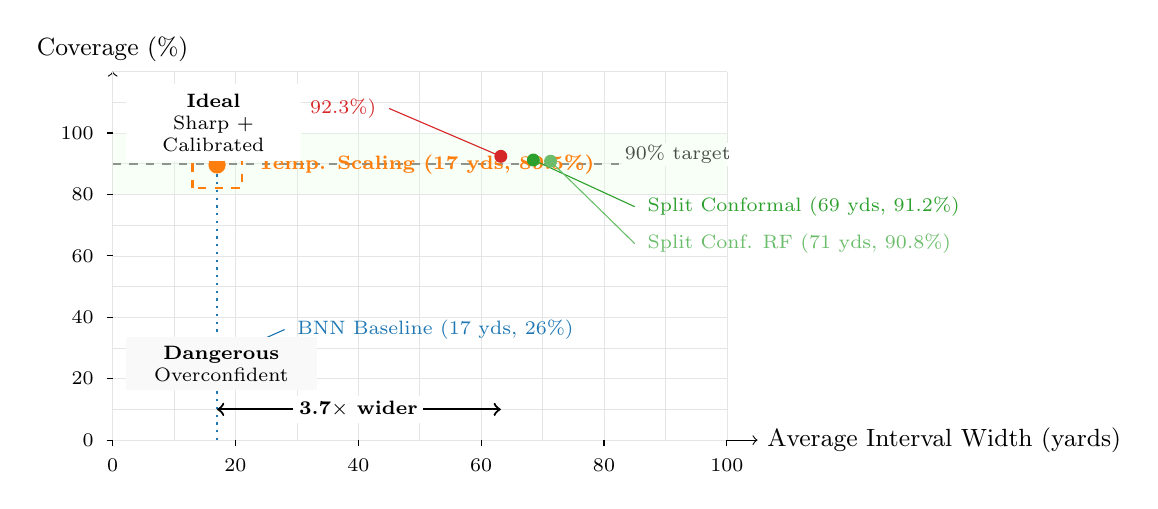
\begin{tikzpicture}[scale=0.78]
  % Load standardized styles
  % tikz_diagram_style.tex - Standardized TikZ diagram styling
% Updated: January 2026 - Publication-ready minimum sizes

% Define accent color (always set to ensure consistency)
\providecolor{accent}{RGB}{31,119,180}

% ---------------------------------------------------
% MINIMUM SIZE STANDARDS (for legibility)
% ---------------------------------------------------
% - Node text: minimum 9pt (\small or \footnotesize)
% - Arrow labels: minimum 8pt (\footnotesize)
% - Box width: minimum 2.5cm for readable text
% - Inner padding: minimum 6pt vertical, 8pt horizontal

% ---------------------------------------------------
% FLOWCHART STYLES
% ---------------------------------------------------

% Standard flowchart box - readable text with adequate padding
\tikzstyle{flowbox}=[
  draw=accent!60,
  rounded corners=4pt,
  line width=0.6pt,
  fill=accent!5,
  text width=3.2cm,           % Increased from 3cm
  minimum height=1.2cm,       % Ensure minimum height
  align=center,
  font=\small,                % Explicit 10pt minimum
  inner ysep=8pt,             % Increased from 6pt
  inner xsep=10pt             % Increased from 8pt
]

% Wide flowbox for longer text (full width)
\tikzstyle{flowbox-wide}=[
  flowbox,
  text width=0.84\linewidth
]

% Narrow flowbox for compact diagrams
\tikzstyle{flowbox-narrow}=[
  flowbox,
  text width=2.5cm,
  font=\footnotesize          % 9pt for narrow boxes
]

% Large flowbox for main components in architecture diagrams
\tikzstyle{flowbox-large}=[
  flowbox,
  text width=4.5cm,
  minimum height=1.5cm,
  font=\normalsize            % 12pt for emphasis
]

% ---------------------------------------------------
% ARROW STYLES
% ---------------------------------------------------

% Standard directional arrow
\tikzstyle{arrow}=[
  ->,
  >=Stealth,                  % Better arrowhead
  line width=0.7pt,           % Slightly thicker for visibility
  color=accent
]

% Thick arrow for emphasis
\tikzstyle{arrow-thick}=[
  arrow,
  line width=1.2pt
]

% Dashed arrow for optional/secondary flows
\tikzstyle{arrow-dashed}=[
  arrow,
  dashed
]

% Bidirectional arrow
\tikzstyle{arrow-bidir}=[
  <->,
  >=Stealth,
  line width=0.7pt,
  color=accent
]

% ---------------------------------------------------
% LABEL AND ANNOTATION STYLES
% ---------------------------------------------------

% Note/callout style - readable annotation
\tikzstyle{note}=[
  font=\footnotesize,         % Increased from \scriptsize (8pt minimum)
  text=black,
  fill=white,
  draw=accent!30,
  rounded corners=3pt,
  inner xsep=4pt,             % Increased from 2pt
  inner ysep=3pt,             % Increased from 1pt
  align=center
]

% Edge label style for arrow annotations
\tikzstyle{edgelabel}=[
  font=\footnotesize,         % 9pt minimum for edge labels
  fill=white,
  inner sep=2pt
]

% ---------------------------------------------------
% ICON AND MARKER STYLES
% ---------------------------------------------------

% Icon circle style
\tikzstyle{icon}=[
  draw=none,
  circle,
  fill=accent!25,
  minimum size=16pt,          % Increased from 13pt
  inner sep=0pt,
  font=\footnotesize\bfseries % Increased from \scriptsize
]

% Numbered step circle
\tikzstyle{stepnum}=[
  circle,
  draw=accent,
  fill=white,
  minimum size=18pt,
  inner sep=0pt,
  font=\footnotesize\bfseries
]

% ---------------------------------------------------
% ARCHITECTURE DIAGRAM STYLES
% ---------------------------------------------------

% Component box for system architecture
\tikzstyle{component}=[
  draw=accent!70,
  rounded corners=6pt,
  line width=0.8pt,
  fill=accent!8,
  text width=4cm,
  minimum height=1.8cm,
  align=center,
  font=\small\bfseries,
  inner sep=10pt
]

% Subcomponent box (nested inside components)
\tikzstyle{subcomponent}=[
  draw=grey5,
  rounded corners=3pt,
  line width=0.5pt,
  fill=white,
  text width=3cm,
  minimum height=1cm,
  align=center,
  font=\footnotesize,
  inner sep=6pt
]

% Database cylinder style
\tikzstyle{database}=[
  cylinder,
  cylinder uses custom fill,
  cylinder body fill=accent!10,
  cylinder end fill=accent!20,
  draw=accent!60,
  minimum width=2cm,
  minimum height=1.5cm,
  font=\small,
  align=center
]

% Cloud/external service style
\tikzstyle{cloud}=[
  draw=grey5,
  fill=grey7!30,
  rounded corners=8pt,
  text width=3cm,
  minimum height=1.2cm,
  align=center,
  font=\small,
  inner sep=8pt
]

% ---------------------------------------------------
% GROUPING AND CONTAINER STYLES
% ---------------------------------------------------

% Container box for grouping related elements
\tikzstyle{container}=[
  draw=grey5,
  dashed,
  rounded corners=6pt,
  line width=0.6pt,
  fill=none,
  inner sep=12pt
]

% Container label
\tikzstyle{containerlabel}=[
  font=\footnotesize\itshape,
  text=grey3,
  anchor=north west
]


  % Define colors
  \definecolor{accent}{RGB}{31,119,180}
  \definecolor{tempcolor}{RGB}{255,127,14}  % Orange
  \definecolor{conformalcolor}{RGB}{44,160,44}  % Green
  \definecolor{cqrcolor}{RGB}{214,39,40}  % Red

  % Axes
  \draw[->] (0,0) -- (10.5,0) node[right, font=\small] {Average Interval Width (yards)};
  \draw[->] (0,0) -- (0,6) node[above, font=\small] {Coverage (\%)};

  % Grid
  \draw[gray!20, very thin] (0,0) grid[xstep=1, ystep=0.5] (10,6);

  % Target coverage line (90%)
  \draw[dashed, thick, black!60] (0,4.5) -- (10,4.5);
  \node[font=\scriptsize, fill=white, inner sep=1pt] at (9.2, 4.65) {90\% target};

  % Acceptable calibration zone (85-95%)
  \fill[green!10, opacity=0.3] (0,4.0) rectangle (10,5.0);

  % BNN baseline interval width reference line
  \draw[dotted, accent, thick] (1.7,0) -- (1.7,5.5);

  % ============================================
  % DATA POINTS (with callout lines to avoid overlap)
  % ============================================

  % BNN Baseline (sharp but under-calibrated) - lower left
  \fill[accent] (1.7, 1.31) circle (3pt);
  \draw[accent, thin] (1.7, 1.31) -- (2.8, 1.8);
  \node[accent, font=\scriptsize, anchor=west] at (2.85, 1.8) {BNN Baseline (17 yds, 26\%)};

  % Temperature Scaling (optimal: sharp AND calibrated) - highlighted
  \fill[tempcolor] (1.7, 4.48) circle (4pt);
  \draw[tempcolor, thick, dashed] (1.3, 4.1) rectangle (2.1, 4.9);
  \node[tempcolor, font=\scriptsize\bfseries, anchor=west] at (2.2, 4.48) {Temp. Scaling (17 yds, 89.5\%)};

  % CQR (adaptive, narrowest conformal) - callout to upper left
  \fill[cqrcolor] (6.32, 4.62) circle (3pt);
  \draw[cqrcolor, thin] (6.32, 4.62) -- (4.5, 5.4);
  \node[cqrcolor, font=\scriptsize, anchor=east] at (4.45, 5.4) {CQR (63 yds, 92.3\%)};

  % Split Conformal (BNN base) - callout to lower right
  \fill[conformalcolor] (6.85, 4.56) circle (3pt);
  \draw[conformalcolor, thin] (6.85, 4.56) -- (8.5, 3.8);
  \node[conformalcolor, font=\scriptsize, anchor=west] at (8.55, 3.8) {Split Conformal (69 yds, 91.2\%)};

  % Split Conformal (RF base) - callout to far right
  \fill[conformalcolor!70] (7.13, 4.54) circle (3pt);
  \draw[conformalcolor!70, thin] (7.13, 4.54) -- (8.5, 3.2);
  \node[conformalcolor!70, font=\scriptsize, anchor=west] at (8.55, 3.2) {Split Conf. RF (71 yds, 90.8\%)};

  % ============================================
  % Sharpness comparison arrows (bottom)
  % ============================================
  \draw[<->, thick, black] (1.7, 0.5) -- (6.32, 0.5);
  \node[font=\scriptsize, fill=white, inner sep=2pt] at (4.0, 0.5) {\textbf{3.7$\times$ wider}};

  % ============================================
  % Axis ticks and labels
  % ============================================
  \foreach \x in {0,20,40,60,80,100} {
    \pgfmathsetmacro{\xpos}{\x/10}
    \draw (\xpos, -0.1) -- (\xpos, 0);
    \node[below, font=\scriptsize] at (\xpos, -0.15) {\x};
  }

  \foreach \y in {0,20,40,60,80,100} {
    \pgfmathsetmacro{\ypos}{\y/20}
    \draw (-0.1, \ypos) -- (0, \ypos);
    \node[left, font=\scriptsize] at (-0.15, \ypos) {\y};
  }

  % ============================================
  % Quadrant labels (corners, non-overlapping)
  % ============================================
  \node[fill=white, text width=2cm, align=center, font=\scriptsize, anchor=north west] at (0.2, 5.8) {
    \textbf{Ideal}\\Sharp + Calibrated
  };

  \node[fill=gray!5, text width=2.2cm, align=center, font=\scriptsize, anchor=south west] at (0.2, 0.8) {
    \textbf{Dangerous}\\Overconfident
  };

\end{tikzpicture}
